\section{Analysis}
\label{sec:analysis}

\subsection{Why Information Asymmetry Helps}
\label{sec:why}

\begin{table}[t]
\centering
\small
\caption{Component ablation (Brier$\,\downarrow$). Each row removes one component from the full system. ``$-$ asymmetry'' gives every agent the full evidence pool ($\rho{=}1$, full sharing) with the same calibrated prompt, i.e., the Standard Debate configuration of our pipeline. Paired 95\% CIs for each removal are given in the text.}
\label{tab:ablation}
\begin{tabular}{lcc}
\toprule
Configuration & \textsc{PolyGym} & FutureX \\
\midrule
InfoDelphi (full) & \textbf{0.1575} & \textbf{0.2006} \\
$-$ calibrated shrink (mean agg.) & 0.1647 & 0.2212 \\
$-$ deliberation (round 1 only) & 0.1698 & --- \\
$-$ information asymmetry & 0.1815 & 0.2433 \\
\bottomrule
\end{tabular}
\end{table}


\paragraph{Component ablation.}
Table~\ref{tab:ablation} removes one component at a time.
Replacing calibrated aggregation with a plain mean costs 0.007 / 0.021 Brier on the two datasets.
Removing deliberation (using round-1 forecasts only) costs 0.005 on \textsc{PolyGym} (paired $\Delta = -0.0052$, CI $[-0.0184, +0.0083]$): the second round helps, but the effect is small relative to question-level noise and not individually significant.
The largest and most robust factor is information structure: giving every agent the full evidence pool with full sharing (the Standard Debate configuration, which shares our prompt and aggregation) degrades the raw ensemble from 0.1647 to 0.1815 on \textsc{PolyGym} (paired $\Delta = -0.0169$, CI $[-0.0314, -0.0029]$) and from 0.2212 to 0.2433 on FutureX ($\Delta = -0.0221$, CI $[-0.0515, +0.0081]$), significant on \textsc{PolyGym} and directionally consistent on FutureX.

\begin{figure}[t]
    \centering
    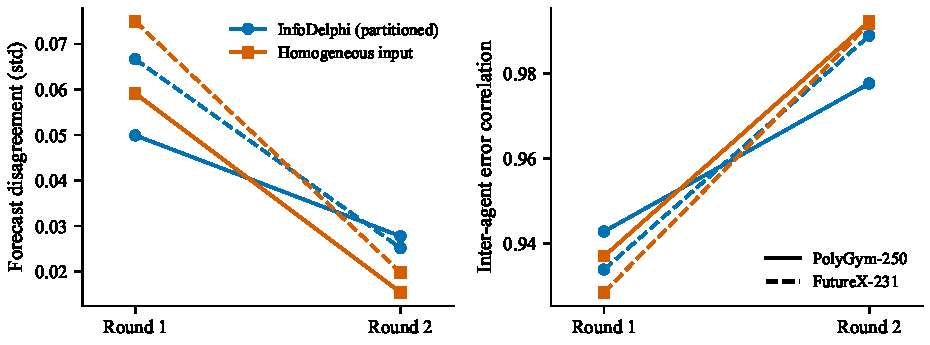
\includegraphics[width=\columnwidth]{figures/fig2_herding.pdf}
    \caption{Deliberation dynamics with and without information asymmetry.
    Left: mean per-question standard deviation of agent forecasts; right: mean
    pairwise inter-agent error correlation. Deliberation under homogeneous input
    collapses forecast diversity (herding); partitioned evidence preserves
    independent signal after deliberation on both datasets.}
    \label{fig:herding}
\end{figure}

\paragraph{Herding dynamics.}
Figure~\ref{fig:herding} traces \emph{how} homogeneous input wastes deliberation.
In round 1, per-question forecast disagreement is comparable for the two information structures (sampling noise dominates).
After one round of deliberation, however, disagreement under homogeneous input collapses by 74--79\% (e.g., 0.059 $\to$ 0.015 on \textsc{PolyGym}), and mean pairwise error correlation rises to 0.99: the panel has effectively merged into a single agent.
With partitioned evidence, agents converge far less (0.050 $\to$ 0.028) and retain a lower error correlation (0.978), preserving the diversity term of Eq.~\eqref{eq:bvd} that ensemble averaging needs.
This is direct empirical evidence for the mechanism behind Proposition~\ref{prop:decorrelation}: what matters is not deliberation itself but whether deliberation has diverse inputs to propagate.

\subsection{Calibration: Aggregation Layer vs.\ Prompt}
\label{sec:calibration_study}

\begin{figure}[t]
    \centering
    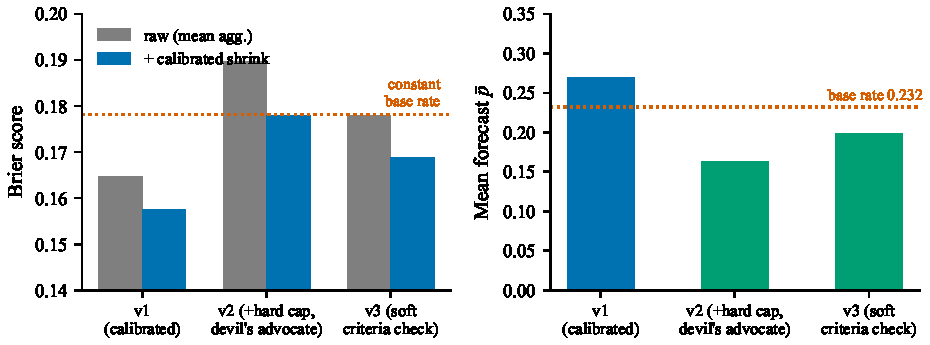
\includegraphics[width=\columnwidth]{figures/fig3_calibration.pdf}
    \caption{Prompt-level vs.\ aggregation-level calibration on
    \textsc{PolyGym}-250. Left: Brier score of three calibration prompts, with and
    without aggregation-level shrinkage; the dotted line is a constant base-rate
    predictor. Right: mean forecast $\bar p$ against the empirical base rate.
    Skeptical prompt wording (v2, v3) depresses the entire forecast distribution
    below the base rate, whereas asymmetric shrinkage corrects overconfidence
    where it occurs.}
    \label{fig:calibration}
\end{figure}

Our agents, like LLM forecasters generally~\citep{tian2023just}, are overconfident on the affirmative side: high-probability YES forecasts hit far less often than stated.
We compared two remedies.
The \emph{prompt-level} route rewrites the forecasting prompt to demand skepticism: v2 adds a devil's-advocate agent and a hard confidence cap; v3 replaces the cap with a soft resolution-criteria checklist.
The \emph{aggregation-level} route keeps the original calibrated prompt (v1) and applies the asymmetric shrinkage of Eq.~\eqref{eq:shrink}.

Figure~\ref{fig:calibration} shows the outcome.
Both prompt interventions \emph{hurt}: v2 degrades raw Brier from 0.1647 to 0.1896 --- worse than predicting the constant base rate (0.1782) --- and v3 lands at 0.1780.
The right panel shows why: prompt-level skepticism cannot be targeted at the overconfident band, so it depresses the whole distribution, pushing the mean forecast from 0.270 down to 0.163 (v2) and 0.198 (v3) against a base rate of 0.232, sacrificing true-YES questions in the mid-band.
Shrinkage applied on top of each prompt improves all three variants, but the best combination by a clear margin is the unmodified prompt plus shrinkage (0.1575).
The parameters fit on Polymarket transfer to FutureX unchanged (0.2212 $\to$ 0.2006, accuracy 0.688 $\to$ 0.701), while re-fitting on FutureX and applying to Polymarket recovers the same setting, indicating the correction captures a model-level bias rather than a dataset artifact.
We conclude that overconfidence corrections belong in the aggregation layer, where they can act asymmetrically on the miscalibrated region, not in the prompt.

\subsection{What Deliberation Cannot Fix}
\label{sec:sports}

\begin{table}[t]
\centering
\small
\caption{Targeted retrieval augmentation on the 106 Sports questions of \textsc{PolyGym}-250 (InfoDelphi full; paired bootstrap vs.\ original evidence, 5{,}000 resamples). Neither augmentation yields a significant improvement.}
\label{tab:sports}
\begin{tabular}{lccc}
\toprule
Evidence & Brier$\,\downarrow$ & AUC$\,\uparrow$ & $\Delta$Brier [95\% CI] \\
\midrule
Original & 0.1908 & 0.696 & --- \\
$+$ opponent identity & 0.1890 & 0.690 & -0.0018 [-0.010, +0.006] \\
$+$ opponent odds/form & 0.1873 & 0.720 & -0.0035 [-0.013, +0.005] \\
\bottomrule
\end{tabular}
\end{table}


Per-domain analysis shows Sports (106 of 250 \textsc{PolyGym} questions) is the weakest domain.
A natural hypothesis is missing information: match-level evidence often lacks the opponent's identity or recent form.
We tested this with two targeted augmentations: decoding the opponent from the market URL slug (adding it as metadata), and retrieving pre-cutoff news about the decoded opponent's odds and form under a three-layer leakage control.
Both augmentations were consumed --- 52--53\% of agent forecasts cite the new documents, and 43\% of retrieved documents contain numeric odds --- yet neither yields a measurable gain (Table~\ref{tab:sports}): paired differences are $-0.002$ and $-0.004$ with CIs straddling zero, and untreated control subsets moved as much as treated ones.
We interpret sports outcomes as evidence-limited at the \emph{model} level: the residual uncertainty is aleatoric given the kind of evidence a text corpus provides, and no amount of deliberation or retrieval within this class of evidence should be expected to remove it.
Information asymmetry improves the \emph{utilization} of informative evidence; it cannot create information the corpus does not contain.
